%%%%%%%%%%%%%%%%%%%%
%
% $Beschreibung: Einleitung in das Projekt "Demonstrator für einen Schrittmotor" $
% $Autor: Grönke $
% $Datum: 09.06.2024 $
% $Pfad: DemonstratorSchrittmotor/DeveloperDoc/Contents/de/Projektbeschreibung.tex $
% $Version: 2 $
%
%
%%%%%%%%%%%%%%%%%%%


\chapter{Projektbeschreibung}

\section{Aufgabenstellung}

Mittels einer Konstruktion, die über einen Schrittmotor verfügt, wird ein Riemen angetrieben. An diesem Riemen ist ein Schlitten befestigt, der durch die Bewegung des Schrittmotors auf einer Linearführung verfahren wird. An dem Gehäuse befindet sich ein Drehschalter, mit dem eine von zehn Bewegungsstufen ausgewählt werden kann. Nach der Auswahl kann das Programm über den grünen Start-Stopp-Knopf gestartet werden. Die Status-LED leuchtet rot, sobald das Gerät einsatzbereit ist. Für die Referenzfahrt wurde ein Endschalter an der Halterung des Schrittmotors befestigt, damit der Schrittmotor auf eine definierte Position referenzieren kann. Es gibt zehn verschiedene Bewegungsstufen. Die Bewegungsstufen unterscheiden sich in der Geschwindigkeit. Pro Stufe wird die Geschwindigkeit erhöht. 

\section{Herausforderungen}

Das Projekt lässt sich in drei verschiedene Teilprojekte unterteilen, die zum Abschluss der Aufgabe führen. Zuerst ist da die Konstruktion des Demonstrators und die hierfür benötigte Auswahl der Hardware-Teile. Vorgabe war, dass der Aufbau nicht zu komplex ist und man sich so auf die wesentlichen Teile konzentriert. Außerdem ist die Arbeit mit der Arduino IDE und die Programmierung des Arduino ein weiterer Teil. Als letzten Punkt ist der Umgang mit den elektronischen Bauteilen zu erwähnen. Der Umgang mit den elektronischen Bauteilen sollte unter großer Vorsicht geschehen, sodass diese nicht durch den elektrischen Strom beschädigt werden. 

\section{Lösungsansatz}
Durch die Ausarbeitung der Herausforderungen, können Lösungsansätze entwickelt werden. Vorab wurde eine erste Konzeptskizze angefertigt, aus der Ideen entstanden. Im ersten Konzept sollte der Schrittmotor eine Plattform über einen Riementrieb axial verfahren, erkennbar in Abbildung \ref{ErsteKonzeptskizze}. Dabei sollte der Verfahrweg der Plattform über einen Abstandssensor mit einem vorher definierten Abstand zu einem Objekt, geregelt werden. Wird das Objekt näher oder weiter entfernt vom Abstandssensor bewegt, verfährt die Plattform mit einem definierten Abstand mit. Alle vorhandenen Bauteile sollten an einem Alu-Profil befestigt werden.

\begin{figure}[htb]
	\begin{center}
		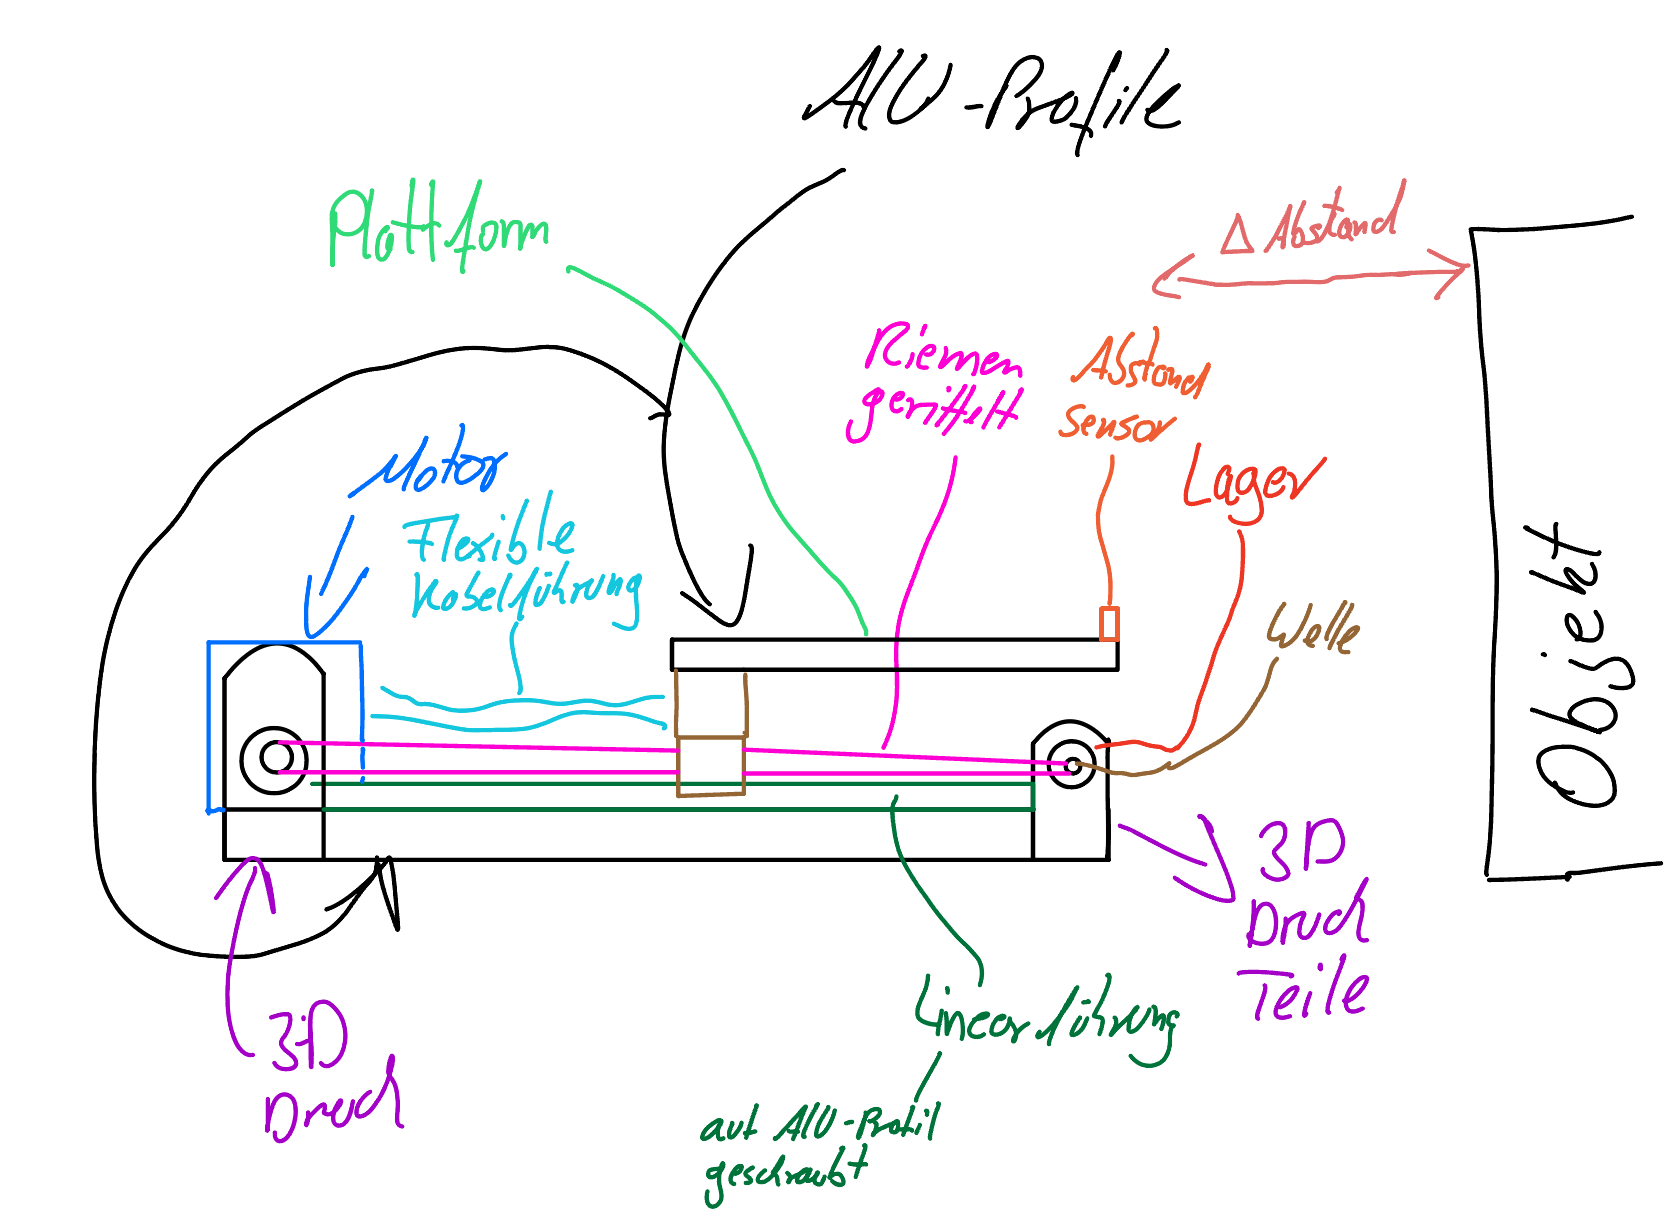
\includegraphics[width=\textwidth]{Images/Konzeptskizze1.png}
		\caption{Erste Konzeptskizze (Eigenaufnahme)} \label{ErsteKonzeptskizze}
\end{center}
\end{figure}

Aufgrund der hohen Komplexität wurde die Plattform inklusive des Abstandssensors, aus dem zweiten Konzept, erkennbar in Abbildung \ref{ZweiteKonzeptskizze}, entfernt. Stattdessen wird auf dem Schlitten der Linearführung ein Zeiger und auf dem Alu-Profil ein Lineal integriert. Mittels verschiedener Stufen soll der Schrittmotor unterschiedliche Bewegungsprofile demonstrieren. Vor allem sollte die Positioniergenauigkeit mit dem Zeiger dargestellt werden. Des Weiteren wurde ein Netzteil integriert, der sowohl den Motor als auch den Arduino mit Spannung versorgt. Außerdem ist ein Schalter zum Ein- und Ausschalten des Demonstrators, ein Stufenschalter zum Auswählen der Stufen sowie ein Taster zum Starten des Demonstrierablaufes eingebaut.  

\begin{figure}[H]
	\begin{center}
		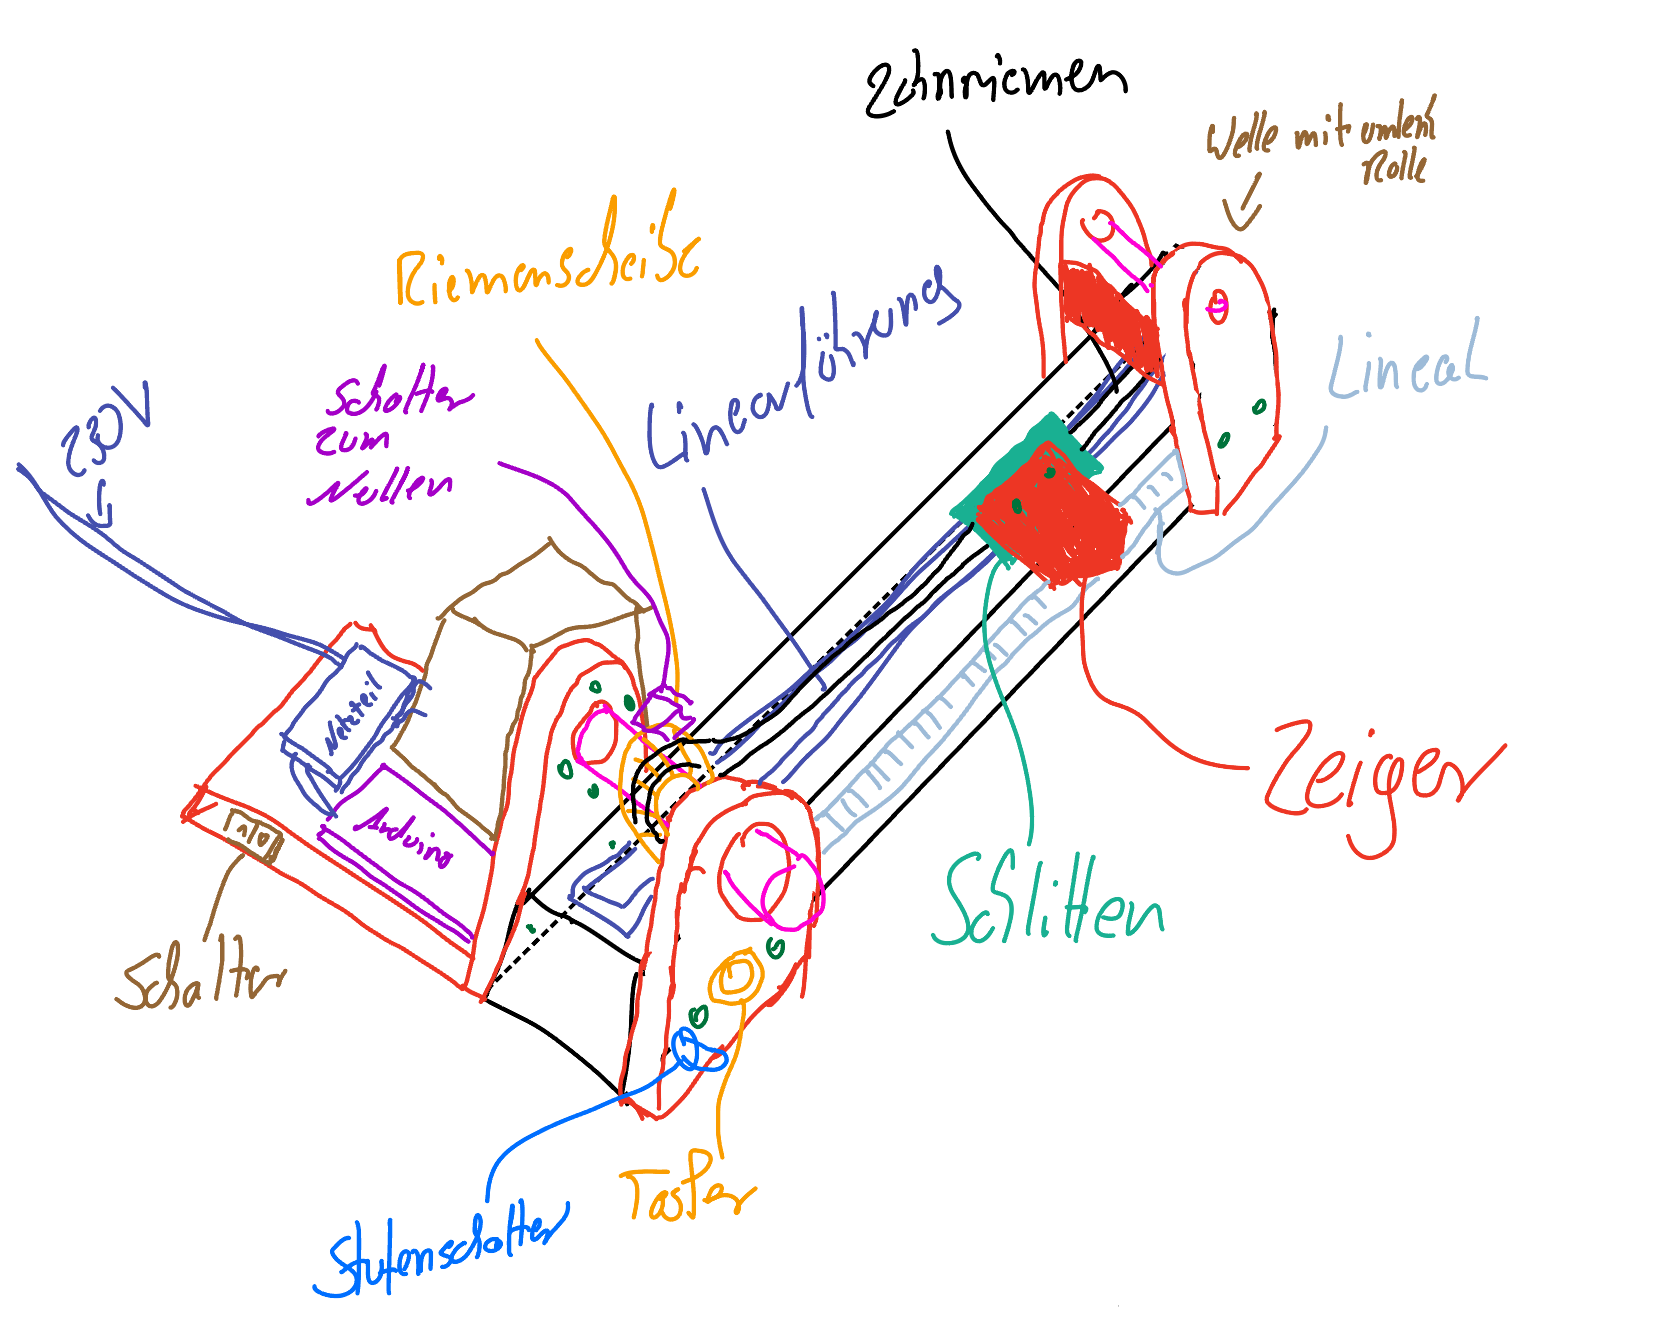
\includegraphics[width=\textwidth]{Images/Konzeptskizze2.png}
		\caption{Zweite Konzeptskizze (Eigenaufnahme)} \label{ZweiteKonzeptskizze}
	\end{center}
\end{figure}

Das zweite Konzept fand gefallen und wurde weiter durchdacht, sodass mit dem Handbuch angefangen werden konnte (siehe Handbuch Demonstrator für einen Schrittmotor). In diesem Handbuch sollte vor allem aus Kundenperspektive die einzelnen Funktionen und die Bedienung geklärt werden. Parallel konnte ein CAD-Modell konstruiert werden, erkennbar in Abbildung \Ref{CADMOD}. Dazu konnte im Team eine MindMap ausgearbeitet werden, die alle möglichen Inhalte und anstehenden Aufgaben zusammenfasst \ref{Mindmap}. Gegenüber dem zweiten Konzept wurde die Hardware aus Transportgründen mit auf dem Aluprofil verlegt und erhielt zum Schutz ein Gehäuse. Des Weiteren konnte eine Materialliste erstellt werden. 

\begin{figure}[H]
	\begin{center}
		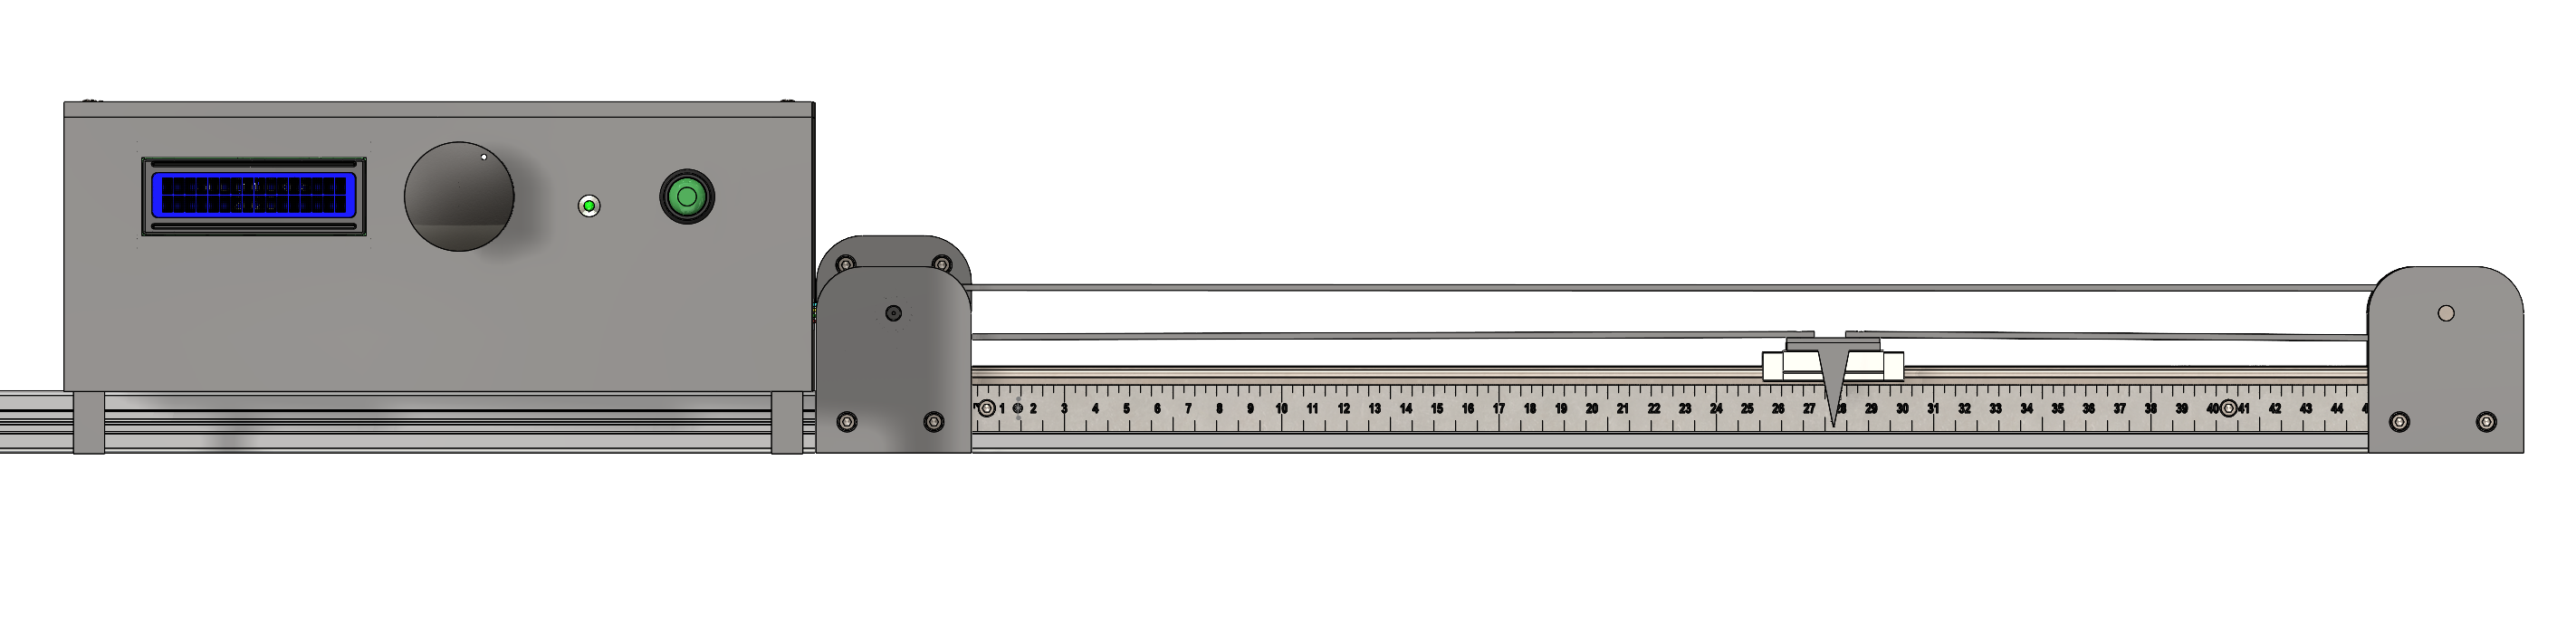
\includegraphics[width=\textwidth]{Images/Konstruktion1.png}
		\caption{CAD-Modell (Eigenaufnahme)} \label{CADMOD}
	\end{center}
\end{figure} 

\begin{figure}[H]
	\begin{center}
		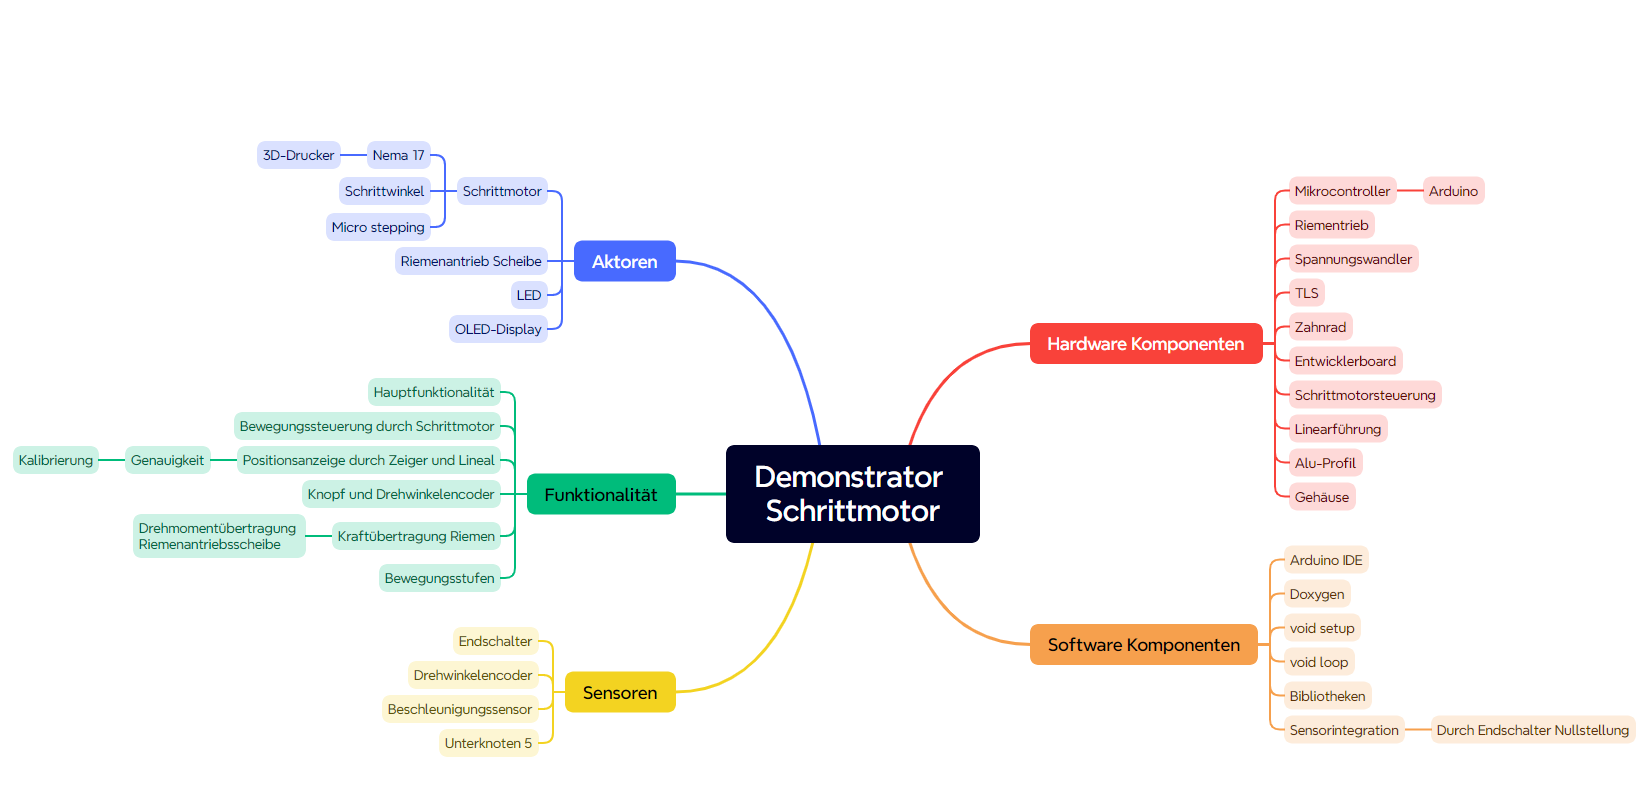
\includegraphics[width=\textwidth]{../Appendix/Mindmap/Mindmap.png}
		\caption{Mindmap} \label{Mindmap}
	\end{center}
\end{figure} 

\section{Anwendungsbereich des Demonstrators}

Die Grundsätzliche Aufgabe des Demonstrators ist die Funktionsweise eines Schrittmotors zu veranschaulichen. Der Demonstrator soll zur Veranschaulichung und als ergänzendes Lehrmittel dienen. So können Schüler und Studierende die Prinzipien der Schrittmotorsteuerung, einschließlich Schrittauflösung und Positionierung praxisnah erlernen. Des Weiteren können Studierende den Demonstrator dazu nutzen, um praktische Erfahrung zu sammeln durch beispielsweise Programmierübungen. Außerdem könnte solch ein Demonstrator als Qualitätskontrolle dienen, um die Leistungsfähigkeit sowie die Genauigkeit von Schrittmotoren zu prüfen und sicherstellen, dass die den erforderlichen Spezifikationen entsprechen. Ein weiteres Anwendungsgebiet können Fachmessen sein, um mit solch einen Demonstrator die Bewegungsabläufe und die präzise Positionierung zu zeigen. 

\section{Besondere Herausforderungen bei den Quellen}

Die größte Herausforderung bei der Beschaffung von Literaturquellen ist die sprachliche Barriere, wenn relevante Quellen nur auf Englisch oder anderen Sprachen verfügbar sind. Diese Barriere Kann das Verständnis und die Interpretation der Quellen erheblich erschweren. Dies führt zu erhöhten Aufwand, da Quellen häufig übersetzt werden müssen. Abhilfe liefern Online-Tools wie Deeple (\href{https://www.deepl.com/de/translator}{www.deepl.com}).
Die fehlende Verfügbarkeit von Datenblättern ist ein weiteres Problem, so stellten Hersteller trotz mehrfacher Nachfrage beim Hersteller keine Datenblätter zur Verfügung. Datenblätter sind für ein für technische Projekte essenziell, da diese wichtige Informationen zur Funktionsweise und Einsatzmöglichkeiten liefern.
Ein weiteres Problem ist das Fehlen vom Herausgabedatum, oder das Altern von Quellen. Dies erschwert eine präzise Dokumentation, da der aktuelle Stand der Technik nicht genau nachzuvollziehen ist. 